\section{问题分析}
\label{sec:analysis}

\subsection{总体思路}
\label{subsec:analysis-overall}

\begin{figure}[H]
  \centering
  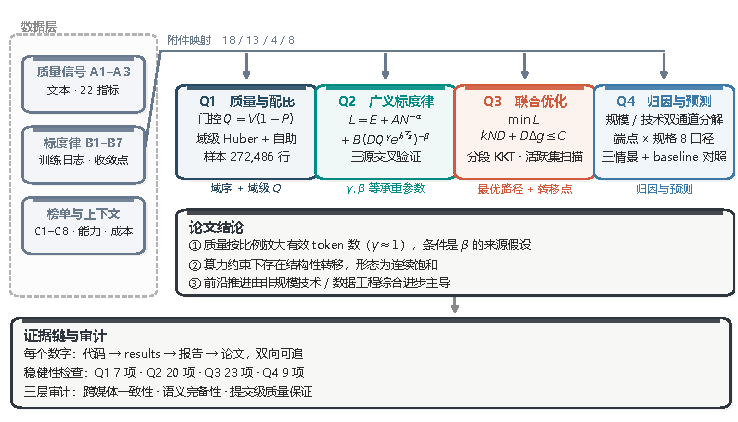
\includegraphics[width=0.98\linewidth]{figures/fig_framework_overall.pdf}
  \caption{四个子问题的研究框架与衔接关系}
  \label{fig:framework-overall}
\end{figure}
四个子问题沿「刻画数据—纳入规律—求解配置—检验外推」的顺序展开，
前一问的输出构成后一问的输入，因此建模设计上需要保证接口的可用性：
问题一输出的质量评分必须定义在可比较的尺度上并能聚合到领域级，
问题二估计的标度律参数必须与问题三的成本约束在单位与量纲上一致，
问题四的预测则要求把损失尺度上的规律可靠地换算到基准得分尺度。
本文的整体框架、各问的方法要点以及证据的追溯路径见图~\ref{fig:framework-overall}。

全文框架。左侧四个分组自上而下对应四个子问题，各组由数据输入连接至方法要点，组间箭头表示相互衔接；
  右侧列出基线对照、敏感性、条件性与外推边界、证据与结论一致性等共同检验。
  数据来自附件 A、B、C 三组，按问映射为 18/13/4/8 个文件。



在方法选择上，本文遵循两条原则。其一是\textbf{可检验优先}：
凡进入主结论的量，都必须给出可机械判定的判据与重抽样区间，
而不是依赖拟合优度的直观好坏。其二是\textbf{退化一致}：
问题二的广义标度律在数据质量取参照值、领域配比取均匀时须退回经典形式，
问题三的最优解在质量不可提升时须退回经典的经验配置，以此作为各自的形式约束。

\subsection{问题一的分析}
问题一包含三项彼此耦合但目标不同的任务，其难点不在于单件技术的复杂度，
而在于三者的口径必须自洽。

质量评价的首要障碍是\textbf{指标方向未在数据中标注}。赛题附录指向《数据说明》给出方向说明，
但该处并无方向标注，因此方向表只能由本队依据字段定义、指标间的一致性与可核验的文本证据推得，
并按可信度分层。其次是\textbf{列表型指标不能取均值}：二分类与有序分类的判别器输出是 logits，
直接取均值会自我抵消，须分别按 logit 差与 softmax 期望类别压缩为标量。
第三是\textbf{长度混淆}：按 token 求和的字段与文档长度高度相关，其表观方向是长度效应的产物。

在合成方式上，本文取「价值组均值 $\times$ 污染组的补」的门控形式，
使两类方向相反的指标各司其职：污染类指标进入门控，从而在合成值上产生乘性惩罚，
而不是与价值类指标在均值中互相抵消。冲突的定义随之自然给出：
\textbf{同一文本在价值维度与污染维度上同时取高分}即为冲突，本文将两个维度分别按分位数锚定，
使冲突率不随样本量漂移。

配比建模的困难来自数据的稀疏性与目标变量的构造。配方表每行中位约有半数的域取精确零，
对数比变换不可用；可用的质量域只有 6 个，与配比域部分不相交。
更关键的是，若以配比加权的域间损失作为目标，配比会同时出现在等式两侧，
构成部分循环。本文的处理是：如实声明该循环，并用简单平均作为对照口径，
以检验域效应的量级排序是否依赖目标口径的选择。

\subsection{问题二的分析}
问题二的形式设计受两条约束牵制。一方面，题目要求新形式在质量取参照值时退回经典标度律，
这排除了把质量作为独立加性项的写法；另一方面，数据条件限制了什么可估：
主拟合数据没有质量变化，配备质量的半合成网格则只有 5 个不同的数据量取值。
这意味着\textbf{数据量指数与质量指数不可在同一份数据上同时良好辨识}，
必须先由真实数据把数据量指数钉住，再由半合成网格反解质量指数。
因此本文采用「先定 $\beta$、后解 $\gamma$」的估计顺序，
并把该顺序的代价——结论对共享假设的依赖——作为一个独立的可检验问题单独报告，
而不是把它藏在拟合过程里。

领域配比项的处理同样受数据限制。全部含配比列的附件中无一与 $(N,D)$ 联合观测，
故配比的效应形状无法跨源验证，只能作为一个声明的承重假设；
相应地，本文对配比项只报告各域边际效应的方向与相对排序，
不报告其绝对量级，因为后者含有一个在该数据条件下严格不可辨识的标度常数。

\subsection{问题三的分析}
问题三是一个带不等式约束的三维非线性规划，但其结构比维度所暗示的更复杂：
探针显示，在九个「预算 $\times$ 成本函数」组合中，最优质量有七个顶在上界，
说明内点一阶条件在多数情形下并不刻画最优解。
因此本文不采用单纯的内点求解，而是\textbf{按活跃约束集分支枚举}：
内点分支与质量触上界的降维分支分别解析求解，再按 KKT 条件筛选，
并用独立数值方法验证分支枚举的完备性。

本问的理论产出在于\textbf{结构性转移的数学定义}。「预算跨越量级时最优策略是否质变」
在没有定义的情况下不可判定，而不同的定义会给出不同的答案。
本文的做法是同时给出三种自然定义并逐一识别，指出哪一种不依赖人为阈值与网格步长，
从而说明「转移存在」这一判断的成立范围——这一点比转移点的具体位置更有价值。

\subsection{问题四的分析}
问题四的核心风险是\textbf{不可检验性}。时间窗口只有 9.1 个月，却要求外推 12–24 个月；
归因分解中的技术通道无法直接观测，只能由规模项之外的残差吸收，
因而它同时包含未观测的数据质量变化与对基准的过拟合，不能被解释为纯粹的算法进步。
本文据此把本问的主辩护对象确定为\textbf{归因侧的方向与量级}：
强调技术通道在全部口径下为正、规模通道的贡献与零不可区分，
而\textbf{不主张任何具体的百分比分割}——后者在端点定义变动下会发生符号翻转。

分解的可辨识性依赖于时间与规模不共线。由于窗口内高分段模型的规模反而在收缩，
规模效应与时间效应在方向上部分背离，这反而有利于二者分离；
但也正因如此，规模项的线性规格会给出符号相反的份额，
本文对规格与端点两种不确定性分别报告，把「点值不稳定」这一事实本身作为结论的一部分。

预测环节还需要把损失尺度上的规律换算到基准得分尺度。
桥接样本中高可比层级只有 7 个点，映射误差与得分尺度同量级，
因此预测区间必然很宽。本文不掩饰这一点，而是把该宽度作为数据条件的结果如实报告，
并同时给出不分解、不外推衰减的纯趋势基线作为对照。

\subsection{关键难点与应对}
\begin{table}[H]
  \centering
  \caption{四个子问题的主要难点与本文的应对方式}
  \label{tab:difficulties}
  \begin{tabular}{@{}p{0.10\linewidth}p{0.42\linewidth}p{0.40\linewidth}@{}}
    \toprule
    子问题 & 主要难点 & 应对方式 \\
    \midrule
    一 & 指标方向无标注；列表型指标不可取均值；长度混淆 & 分层方向表并报敏感性；
      logit 差与 softmax 期望类别压缩；逐 token 归一化 \\
    一 & 配方表稀疏且质量域部分不相交；目标含配比、存在循环 & 不施对数比变换；
      显式声明循环并给出对照口径 \\
    二 & 质量指数与数据量指数不可同时辨识；配比效应形状不可跨源验证 &
      先定数据量指数、后解质量指数；只报配比效应的方向与排序 \\
    三 & 最优解多数触上界，内点条件不刻画最优 & 按活跃约束集分支枚举，
      并以独立数值方法验证完备性 \\
    三 & 「结构性转移」无公认定义 & 并报三种定义，标明哪一种不依赖阈值与步长 \\
    四 & 窗口不足以外推；技术通道不可直接观测 & 主辩护改为方向与量级，
      不主张百分比分割；技术通道只作综合表述 \\
    四 & 损失与得分尺度之间的映射样本极少 & 映射误差作独立随机项传播，
      并给出纯趋势基线对照 \\
    \bottomrule
  \end{tabular}
\end{table}
